\chapter{TÌM HIỂU CÁC LINH KIỆN KHÁC}
    \section{Bộ điều chỉnh LM2576}
        \subsection{Giới thiệu}
            \hspace*{0.6cm}LM2576 là một bộ điều chỉnh điện áp chuyển mạch (switching regulator) hiệu suất cao, có thể cung cấp dòng điện lên đến 3A. Nó được thiết kế để giảm thiểu số lượng linh kiện ngoại vi và đơn giản hóa thiết kế mạch.
        \subsection{Đặc điểm kỹ thuật}
            \begin{itemize}
                \item Điện áp đầu vào: 4V đến 40V
                \item Điện áp đầu ra: 1.23V đến 37V
                \item Dòng điện đầu ra: lên đến 3A
                \item Hiệu suất chuyển đổi: lên đến 90%
                \item Tần số chuyển mạch: 52kHz
            \end{itemize}   
        \subsection{Sơ đồ chân}
            \begin{figure}[H]
                \centering
                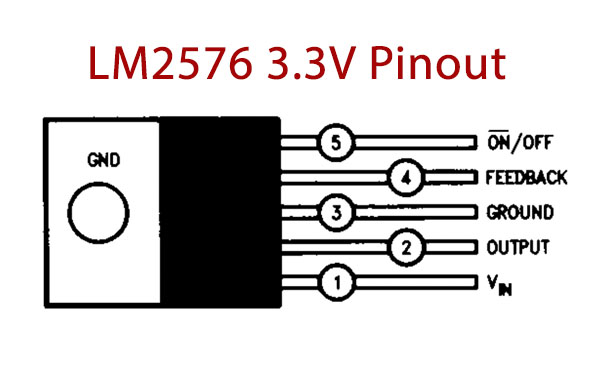
\includegraphics[width=0.5\textwidth]{pictures/lm2576_pinout.png}
                \caption{Sơ đồ chân của LM2576}
            \end{figure}
        \subsection{Chức năng từng chân của LM2576}
            LM2576 có 5 chân với các chức năng như sau:
            
            \begin{itemize}
                \item \textbf{Chân 1 (VIN)}: Chân này là đầu vào điện áp. Điện áp đầu vào có thể dao động từ 4V đến 40V.
                \item \textbf{Chân 2 (Output)}: Chân này là đầu ra điện áp đã được điều chỉnh. Điện áp đầu ra có thể được điều chỉnh từ 1.23V đến 37V tùy thuộc vào cấu hình mạch.
                \item \textbf{Chân 3 (Ground)}: Chân này là chân nối đất (GND) của mạch.
                \item \textbf{Chân 4 (Feedback)}: Chân này được sử dụng để điều chỉnh điện áp đầu ra. Nó nhận tín hiệu phản hồi từ mạch để duy trì điện áp đầu ra ổn định.
                \item \textbf{Chân 5 (ON/OFF)}: Chân này được sử dụng để bật hoặc tắt bộ điều chỉnh. Khi chân này được kéo lên mức cao, bộ điều chỉnh sẽ tắt và khi kéo xuống mức thấp, bộ điều chỉnh sẽ bật.
            \end{itemize}

            
        \subsection{Ứng dụng}
            LM2576 được sử dụng rộng rãi trong các ứng dụng như:
            \begin{itemize}
                \item Bộ nguồn chuyển mạch
                \item Bộ điều chỉnh điện áp cho các thiết bị điện tử
                \item Hệ thống cung cấp điện cho vi điều khiển và các mạch số
            \end{itemize}
            
        \subsection{Sơ đồ mạch ứng dụng}
            \begin{figure}[H]
                \centering
                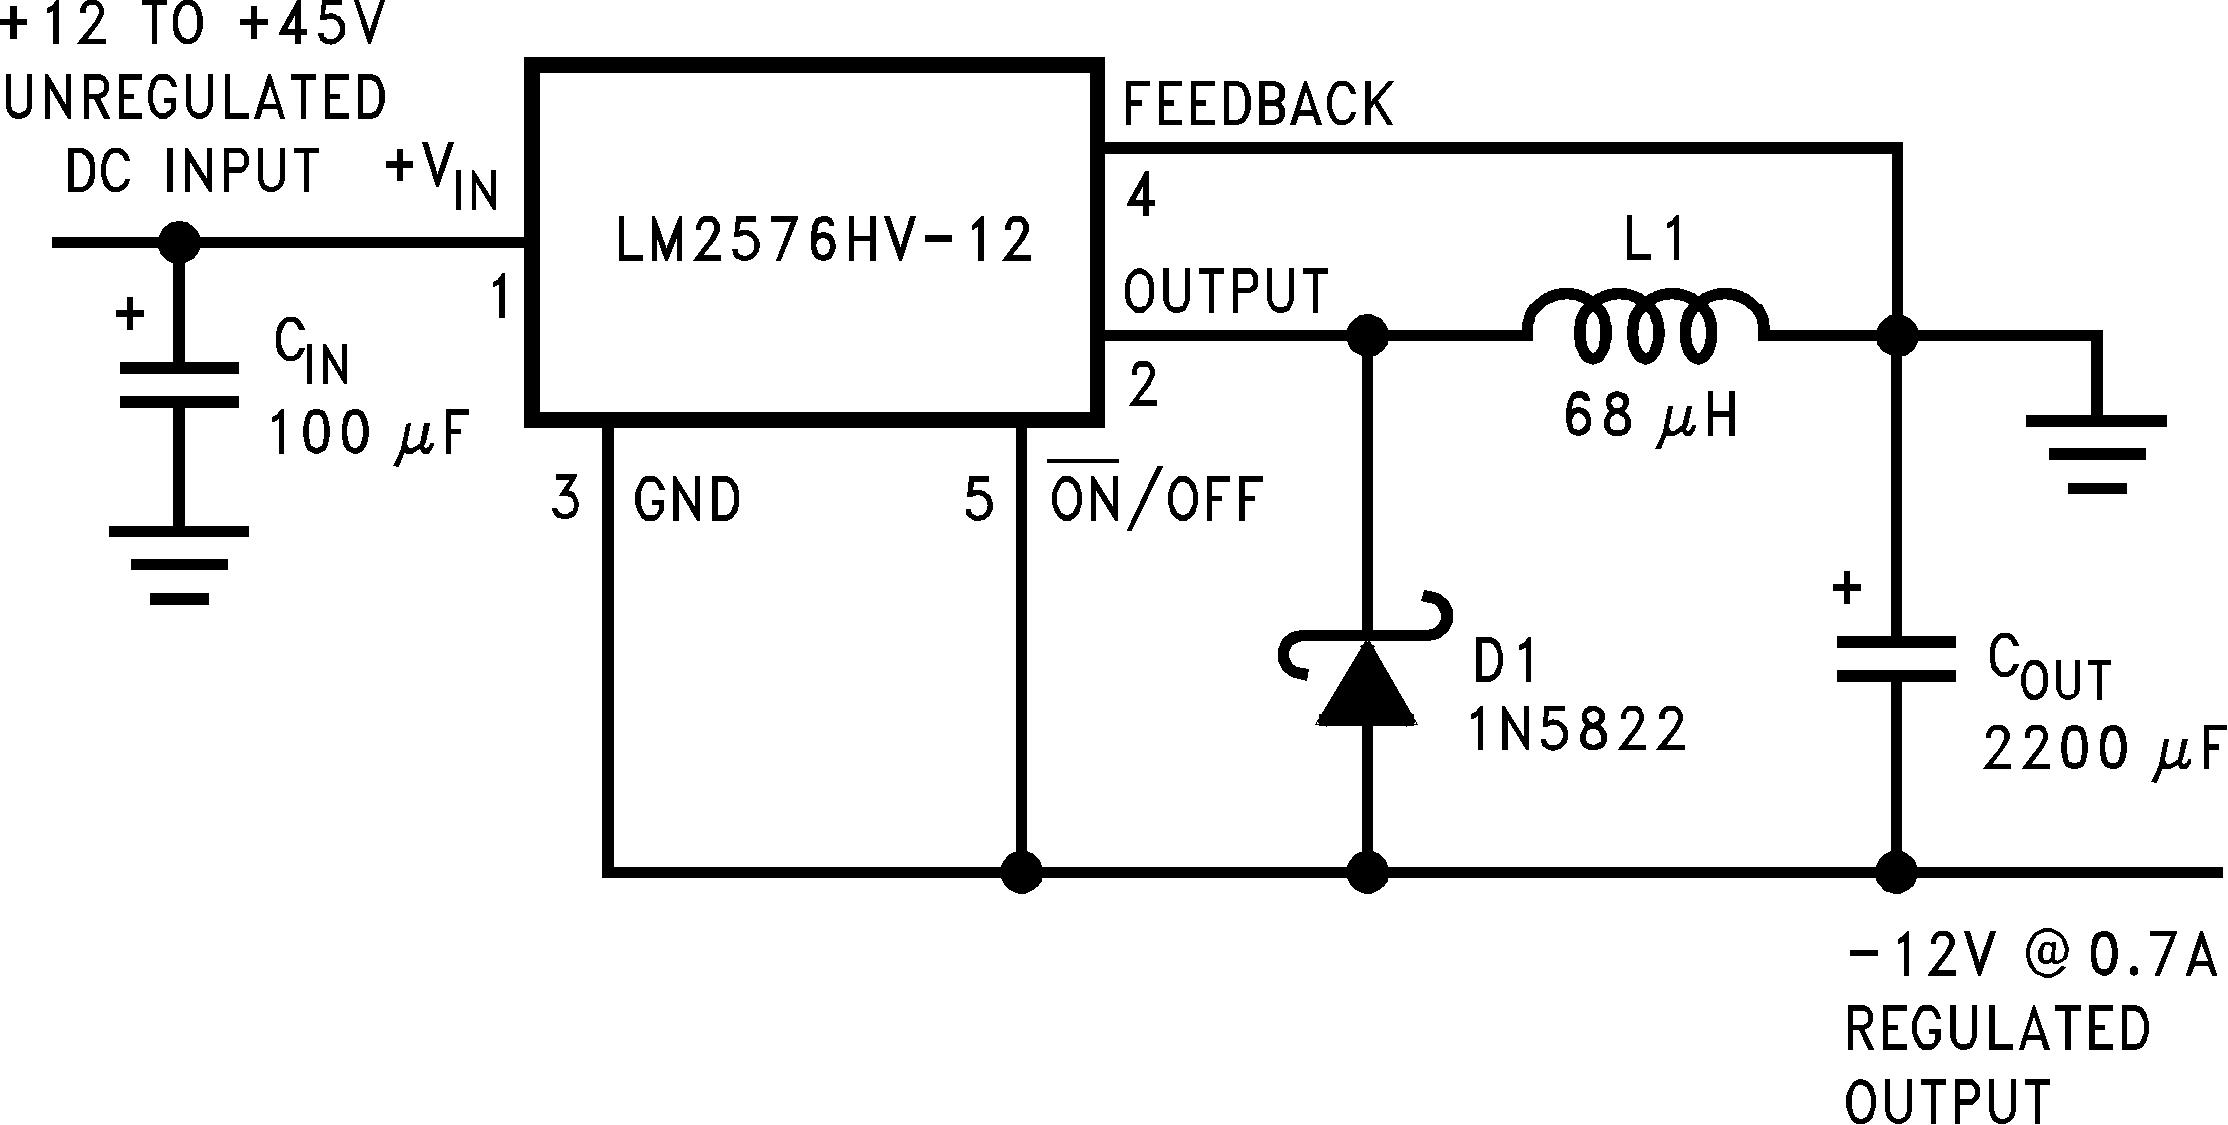
\includegraphics[width=0.8\textwidth]{pictures/lm2576_application_circuit.png}
                \caption{Sơ đồ mạch ứng dụng của LM2576}
            \end{figure}

        \subsection{Giải thích chức năng của mạch ứng dụng}
            \hspace*{0.6cm}Sơ đồ mạch ứng dụng của LM2576 bao gồm các thành phần chính như sau:
            
            \begin{itemize}
                \item \textbf{LM2576}: Bộ điều chỉnh điện áp chuyển mạch, là thành phần chính của mạch.
                \item \textbf{Cuộn cảm (L)}: Lưu trữ năng lượng khi transistor bên trong LM2576 bật và giải phóng năng lượng khi transistor tắt, giúp duy trì điện áp đầu ra ổn định.
                \item \textbf{Tụ điện đầu vào (C\textsubscript{in})}: Giúp lọc nhiễu và ổn định điện áp đầu vào.
                \item \textbf{Tụ điện đầu ra (C\textsubscript{out})}: Giúp lọc nhiễu và ổn định điện áp đầu ra.
                \item \textbf{Điện trở phản hồi (R\textsubscript{fb})}: Được sử dụng để điều chỉnh điện áp đầu ra bằng cách cung cấp tín hiệu phản hồi cho chân Feedback của LM2576.
                \item \textbf{Diode Schottky (D)}: Giúp chuyển đổi năng lượng từ cuộn cảm sang tải khi transistor bên trong LM2576 tắt.
            \end{itemize}
            
            \textbf{Nguyên lý hoạt động}:
            \begin{enumerate}
                \item Khi LM2576 bật, transistor bên trong dẫn điện, dòng điện chạy qua cuộn cảm (L) và lưu trữ năng lượng trong đó.
                \item Khi LM2576 tắt, transistor ngừng dẫn điện, năng lượng lưu trữ trong cuộn cảm được giải phóng qua diode Schottky (D) để cung cấp cho tải.
                \item Tụ điện đầu ra (C\textsubscript{out}) giúp làm mịn điện áp đầu ra, đảm bảo điện áp ổn định cho tải.
                \item Điện trở phản hồi (R\textsubscript{fb}) cung cấp tín hiệu phản hồi cho chân Feedback của LM2576 để điều chỉnh điện áp đầu ra theo giá trị mong muốn.
            \end{enumerate}
            
        \subsection{Nguyên lý hoạt động}
            LM2576 hoạt động dựa trên nguyên lý chuyển mạch, sử dụng một transistor công suất để điều chỉnh điện áp đầu ra. Khi transistor này bật, năng lượng được lưu trữ trong cuộn cảm. Khi transistor tắt, năng lượng này được giải phóng để cung cấp cho tải.
            
        \subsection{Lưu ý khi sử dụng}
            \begin{itemize}
                \item Đảm bảo các linh kiện ngoại vi như cuộn cảm, tụ điện được chọn đúng giá trị để đảm bảo hiệu suất hoạt động.
                \item Kiểm tra nhiệt độ của LM2576 trong quá trình hoạt động để tránh quá nhiệt.
                \item Sử dụng tản nhiệt nếu cần thiết để đảm bảo LM2576 hoạt động ổn định.
            \end{itemize}
    \section{Mô-đun điều khiển động cơ BTS7960B}     
        \subsection{Giới thiệu}
            BTS7960B là một mô-đun điều khiển động cơ H-Bridge công suất cao, có thể điều khiển dòng điện lên đến 43A. Nó được thiết kế để điều khiển động cơ DC trong các ứng dụng công nghiệp và tự động hóa.
            
            \section{Đặc điểm kỹ thuật}
            \begin{itemize}
                \item Điện áp đầu vào: 5.5V đến 27V
                \item Dòng điện đầu ra: lên đến 43A
                \item Bảo vệ quá nhiệt và quá dòng
                \item Điều khiển tốc độ động cơ bằng PWM
            \end{itemize}
            
        \subsection{Sơ đồ chân}
            \begin{figure}[H]
                \centering
                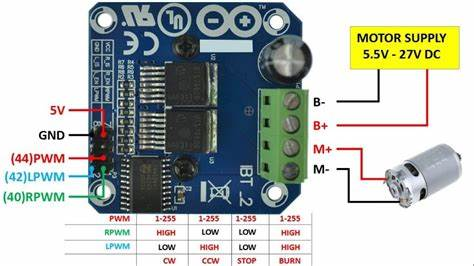
\includegraphics[width=0.5\textwidth]{pictures/bts7960b_pinout.png}
                \caption{Sơ đồ chân của BTS7960B}
            \end{figure}
            
        \subsection{Ứng dụng}
            BTS7960B được sử dụng rộng rãi trong các ứng dụng như:
            \begin{itemize}
                \item Điều khiển động cơ DC công suất cao
                \item Robot tự động
                \item Hệ thống điều khiển chuyển động
            \end{itemize}
            
        \subsection{Sơ đồ mạch ứng dụng}
            \begin{figure}[H]
                \centering
                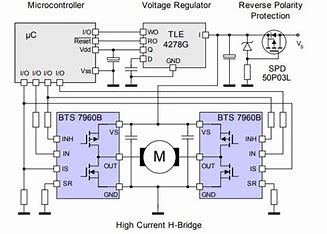
\includegraphics[width=0.8\textwidth]{pictures/bts7960b_application_circuit.png}
                \caption{Sơ đồ mạch ứng dụng của BTS7960B}
            \end{figure}
            
        \subsection{Nguyên lý hoạt động}
            BTS7960B hoạt động dựa trên nguyên lý H-Bridge, cho phép điều khiển chiều quay và tốc độ của động cơ DC bằng cách điều chỉnh tín hiệu PWM.
            
        \subsection{Chức năng từng chân của BTS7960B}
            BTS7960B có các chân với các chức năng như sau:
            
            \begin{itemize}
                \item \textbf{VCC}: Chân cấp nguồn cho mô-đun.
                \item \textbf{GND}: Chân nối đất của mô-đun.
                \item \textbf{RPWM}: Tín hiệu PWM điều khiển chiều quay phải của động cơ.
                \item \textbf{LPWM}: Tín hiệu PWM điều khiển chiều quay trái của động cơ.
                \item \textbf{R\_EN}: Kích hoạt chiều quay phải của động cơ.
                \item \textbf{L\_EN}: Kích hoạt chiều quay trái của động cơ.
                \item \textbf{R\_IS}: Giám sát dòng điện chiều quay phải.
                \item \textbf{L\_IS}: Giám sát dòng điện chiều quay trái.
            \end{itemize}
            
        \subsection{Giải thích chức năng của mạch ứng dụng}
            Sơ đồ mạch ứng dụng của BTS7960B bao gồm các thành phần chính như sau:
            
            \begin{itemize}
                \item \textbf{BTS7960B}: Mô-đun điều khiển động cơ H-Bridge, là thành phần chính của mạch.
                \item \textbf{Động cơ DC}: Được điều khiển bởi mô-đun BTS7960B.
                \item \textbf{Nguồn cấp}: Cung cấp điện áp và dòng điện cần thiết cho mô-đun và động cơ.
                \item \textbf{Tín hiệu điều khiển (PWM)}: Điều khiển tốc độ và chiều quay của động cơ.
            \end{itemize}
            
            \textbf{Nguyên lý hoạt động}:
            \begin{enumerate}
                \item Tín hiệu PWM được gửi đến các chân RPWM và LPWM để điều khiển tốc độ và chiều quay của động cơ.
                \item Các chân R\_EN và L\_EN được sử dụng để kích hoạt chiều quay phải và trái của động cơ.
                \item Các chân R\_IS và L\_IS giám sát dòng điện qua động cơ để bảo vệ quá dòng.
            \end{enumerate}
            
            \end{document}